\documentclass[10pt]{article}

\usepackage[utf8]{inputenc}
\usepackage{amsmath, amssymb}
\usepackage{graphicx}
\usepackage{cite}
\usepackage{hyperref}
\usepackage{geometry}
\geometry{margin=1in}

\setlength{\parindent}{0pt}
\setlength{\parskip}{0.5em}

\title{Evaluating CNN performance on birdCLEF 2025}
\author{
  Tommaso Ferracina\
  \and
  Tebe Nigrelli
}
\date{\today}


\begin{document}

\maketitle

\begin{abstract}
  Mobile and habitat-diverse animal species are valuable indicators of biodiversity change, as shifts in their population signal the success or failure of ecological restoration efforts. Conducting "on the ground" biodiversity surveys is costly and logistically demanding, so conservation campaigns have opted for autonomous recording units to record audio data in the field. Through modern machine learning techniques, these audio samples can be processed and analyzed to better understand the restoration effort's impact on local biodiversity. In this investigation, we tackle the BirdCLEF 2025 sound recognition strategy by building a classifier to detect bird calls in complex, multi-label audio recordings. Our approach integrates audio preprocessing with various implementations of convolutional neural networks (CNN), training on log-mel spectrograms, as well as using semi-supervised learning. We mitigate noise and class imbalance through label smoothing and data augmentation. We concluded our investigation by evaluating our methodology and model performance, and submitting our final models for evaluation on the competition scoreboard.
\end{abstract}

\section*{Description of the Task}

In this investigation, we compared the performance of different architectures for the BirdCLEF2025 Kaggle competition \cite{birdclef2025}, hosted by the Cornell Lab of Ornithology. The Lab supplies labeled audio clips originating from three different collection of species audio: \textit{iNaturalist}, \textit{Xeno-Canto} and the \textit{Colombian Sound Archive}. The audios contain various animal species, ranging from four different taxonomy classes: Insecta, Amphibia, Mammalia, and Aves. In addition to this, unlabeled Soundscapes are also provided to be used for unsupervised learning. The final objective is to develop a model capable of analyzing unseen Soundscapes to accurately detect and classify the species within.

\section*{Exploratory Data Analysis}

The audio data consists of \texttt{.ogg} files alongside metadata in a corresponding \texttt{.csv} file. The main source of species information is found in the \texttt{taxonomy.csv} file, where the primary label name is linked to the animals common name, scientific name, and the animal class they belong to.

The labeled training samples are stored in the \texttt{train\_audio} folder, where each species has a dedicated subfolder named after its ID, containing all corresponding audio clips. This data is completely described by the \texttt{train.csv}, which provides key metrics on each recording, such as the source, recording location, primary label, and some secondary labels are present, which identify other species that may also be present in the audio, though with a lower reliability.

Finally, the soundscapes are stored in the \texttt{train\_soundscapes} folder and labeled by date and ID. Each soundscapes is exactly a minute long, while the audio samples had variable length. All audio files metrics were provided in a normalized format, fitted the same audio range: $72$ as bitrate, a sample rate of $32000$, $1$ channel and \textit{vorbis} as audio codec.

\section*{Audio Durations}

The \textit{labeled} dataset is composed of '28564' audio files, totalling '280' hours of audio, whereas the \textit{soundscape} '9726' for a total of '162' hours.

\begin{table}[h!]
  \centering
  \begin{tabular}{|l|r|r|}
    \hline
    & \textbf{labeled} & \textbf{Unlabeled} \\
    \hline
    Mean                  & 35s      & 60 s       \\
    Number of Samples      & 28,564   & 9,726      \\
    Modal Duration (10 s)  & 0--10s   & 60s        \\
    Total Duration         & 280h     & 162.1 h    \\
    \hline
  \end{tabular}
\end{table}

It should be noted that although labeled data is larger in sum, there are (relatively) few usable samples, due to the vast number of labels and many labeled audio clips containing just a few seconds of relevant sound, followed by the spoken description of the recording setup and specifications: a minute-long recording may provide as little as 5 seconds of relevant audio. 

\begin{minipage}{0.48\linewidth}
Although at that stage we could not infer what portion of the dataset was actually of use, we showed the histogram of duration, comparing frequency to audio duration. Notably, frequency had to be rescaled on a log scale, and although the vast majority of the audio samples were short (64\% of recordings were shorter than 30 seconds), some outliers were present (25 and 29 minutes long audios).
\end{minipage}
\hfill
\begin{minipage}{0.48\linewidth}
  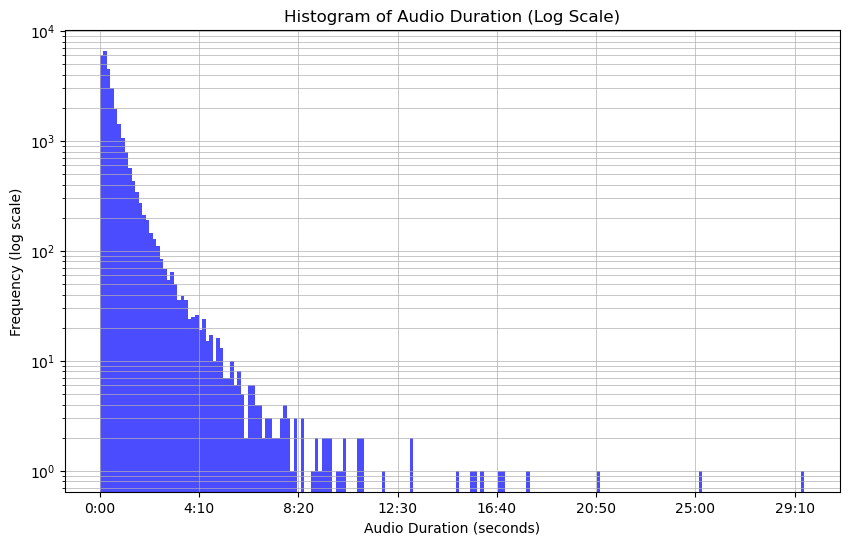
\includegraphics[width=\linewidth]{img/training_duration_histogram.png}
\end{minipage}

\section*{Label Distribution}

\begin{minipage}{0.48\linewidth}
The main labels of focus are the 'primary' labels which are singular. All the clips also have a 'secondary' column which can either be empty or hold a list of other species which can be heard in the recording. Finally, the 'type' column, if present, describes the type of bird call recorded. We considered first the distribution of primary labels in the dataset, immediately noticing an inverse relation between label presence and label rank.
\end{minipage}
\hfill
\begin{minipage}{0.48\linewidth}
  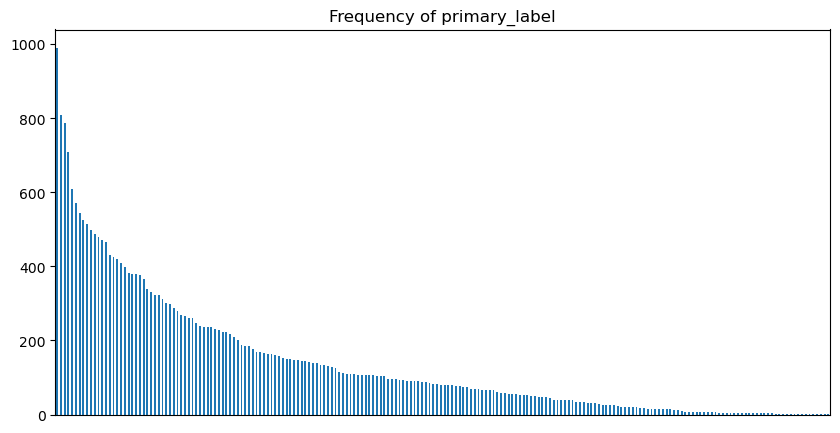
\includegraphics[width=\linewidth]{img/train_primary_histogram.png}
\end{minipage}

\vspace{1em}

\begin{minipage}{0.48\linewidth}
Moreover, most secondary labels are empty. This is apparent in the following sand graph: each column represents a primary label, and the pile of colors shows how many of each secondary label are present in the recordings with the given primary label value. Notably, most secondary labels are empty, as can be seen in the large uniform area.
\end{minipage}
\hfill
\begin{minipage}{0.48\linewidth}
  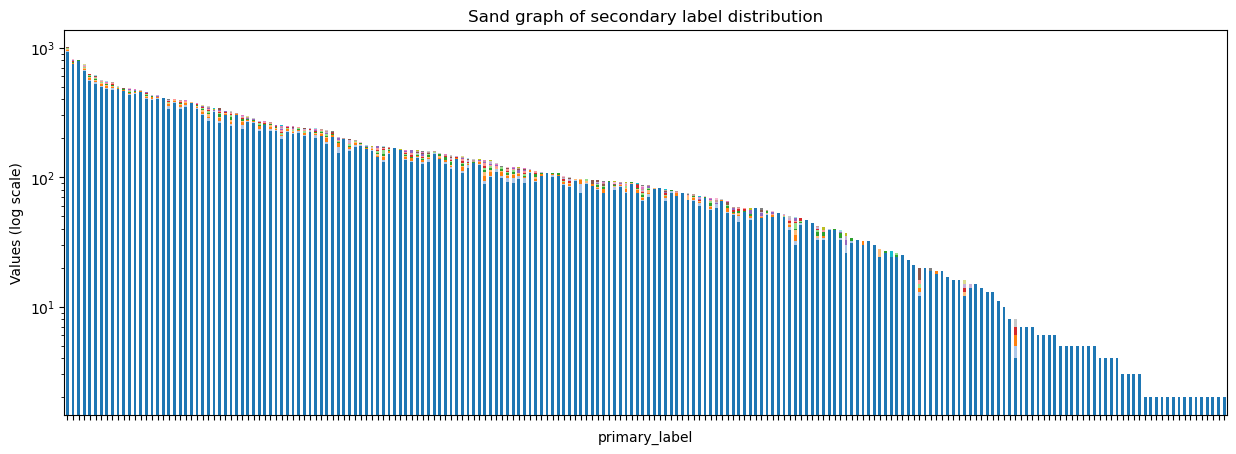
\includegraphics[width=\linewidth]{img/train_secondary_sand.png}
\end{minipage}

\vspace{1em}

\begin{minipage}{0.48\linewidth}
Discarding the empty secondary label, we observed more closely the richness in variety: these are few secondary labels, distributed among various primary labels.
\end{minipage}
\hfill
\begin{minipage}{0.48\linewidth}
  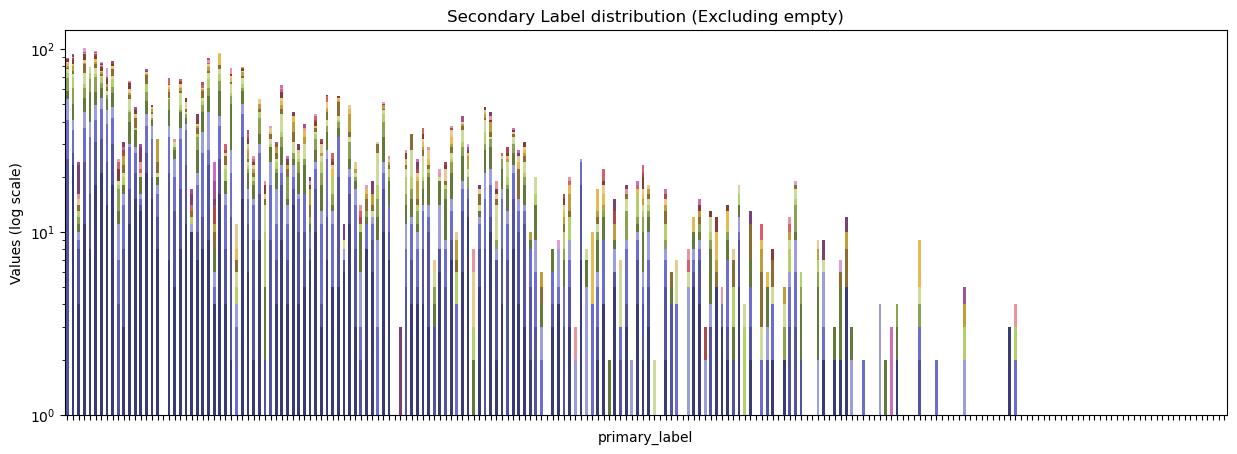
\includegraphics[width=\linewidth]{img/train_secondary_sand_nonempty.png}
\end{minipage}

\vspace{1em}

\begin{minipage}{0.48\linewidth}
The final column of classification information, \texttt{type}, specifies a list of qualitative descriptions of the results: although most frequent labels are, in the following order: \textit{song}, \textit{no type}, \textit{call}, \textit{flight call} and \textit{alarm call}, there is a rich variety of calls, with 587 unique, which are sparsely represented in the data.
\end{minipage}
\hfill
\begin{minipage}{0.48\linewidth}
  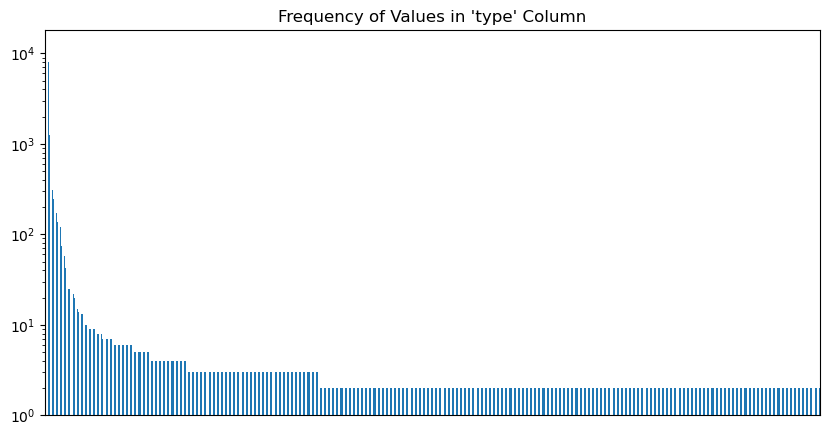
\includegraphics[width=\linewidth]{img/train_type_histogram.png}
\end{minipage}

\section*{Data Sources}

The dataset consists of audio recordings from three different sources: Xeno-Canto, a global bird sound repository; iNaturalist, a citizen science platform with diverse wildlife recordings; and the Colombian Sound Archive, a national collection preserving Colombia's acoustic biodiversity. These sources vary in their level of scientific rigor, as some are curated by experts, while others are maintained by hobbyists. Due to this, we quickly identified several data quality challenges. For example, there is inconsistent availability of quality ratings across sources, with only Xeno-Canto providing such ratings. Moreover, a high variability in audio quality affects model performance, since recordings often contain silence, background noise, and other irrelevant sounds. There is also a risk of losing representation for rare species during data cleaning or filtering, compounded by a severe class imbalance.

\section*{Challenges with the Data}

Some audio samples in the labeled dataset are spliced with human voices explaining the microphone setup. Moreover, some audio recordings contain large proportions of static noise, with no relevant information in those cases.

\begin{minipage}{0.7\linewidth}
The labeled recordings are characterized by an extreme degree of class imbalance in training data, with the least catalogued classes being composed of less than a minute samples in total.Although the audio recordings are labeled by a reliable \texttt{primary\_label} feature, we also have access to a less reliable set of secondary labels. This motivated us to consider different levels of trustworthiness for the secondary labels, which we explored through the use of the m parameter, obtaining a range of accuracies in our models.

On a final note, almost half of the dataset is unlabeled, which can be used to extract more information on the characteristics of audio data, withou additional information through labelling.
\end{minipage}
\hfill
\begin{minipage}{0.3\linewidth}
  \centering
  \begin{tabular}{|r|l|}
    \hline
    \textbf{primary\_label} & \textbf{Tot} \\
    \hline
    81930    & 44 sec \\
    67082    & 44 sec \\
    548639   & 29 sec \\
    66016    & 26 sec \\
    523060   & 24 sec \\
    868458   & 23 sec \\
    42113    & 22 sec \\
    42087    & 21 sec \\
    21116    & 13 sec \\
    1564122  & 11 sec \\
    \hline
  \end{tabular}
\end{minipage}

\section*{Audio Preprocessing}

To make the analysis computationally tractable, we experimented with transformations that transform raw audio into spectrogram representations. The most used method for this in deep learning is the \emph{Mel spectrogram}\cite{mel_cepstrum}. The Mel spectrogram applies a Mel filter bank to a \emph{short-time Fourier transform} (STFT), mapping frequencies to the Mel scale, defined in terms of perceived pitch and modeled after human auditory perception. Compared to raw spectrograms, the Mel representation reduces dimensionality and increases robustness to noise and variability. 


\begin{center}
  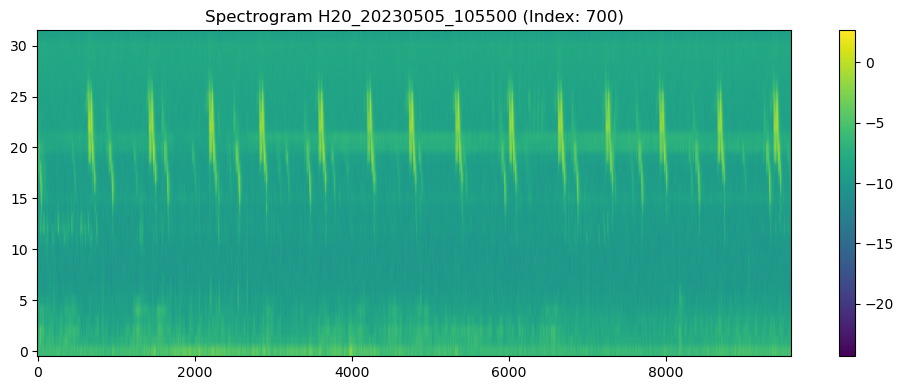
\includegraphics[width=0.7\linewidth]{img/scape_spectrogram.png}
\end{center}

\section*{Audio Splicing}

The final classification task involves identifying bird species present within a one-minute audio recording. To achieve this, we divided the recording into smaller segments, classifying the species detected in each segment. We chose a 5-second window size, meaning our model is trained on 5-second chunks of labeled data. All the recordings in the dataset were preprocessed accordingly: audios longer than 5 seconds were split into multiple segments, while recordings shorter than 5 were zero-padded. In cases of a leftover segment of at least 2.5 seconds (e.g., an 8-second recording), we included both the first and last 5-second segments, aligning the remaining audio to the end.

\subsection*{Clustering for Audio Segmentation}

Since labeled audios often include sources of external noise, which does not correspond to any relevant label, we were interested in removing the worst examples in the training data to improve the quality of the dataset. This transformation would produce a classifier model on only the best data. We explored this direction by evaluating the performance of different clustering algorithms:

\begin{minipage}{0.6\linewidth}
\textit{K-means}: the simplest conceptually, performed reasonably well, though it involved the added difficulty of assigning the number of clusters beforehand. Despite using the number of primary and secondary labels, together with a 'null' label as a reference for the number of clusters, we were not able to improve the grouping.
\end{minipage}
\hfill
\begin{minipage}{0.35\linewidth}
  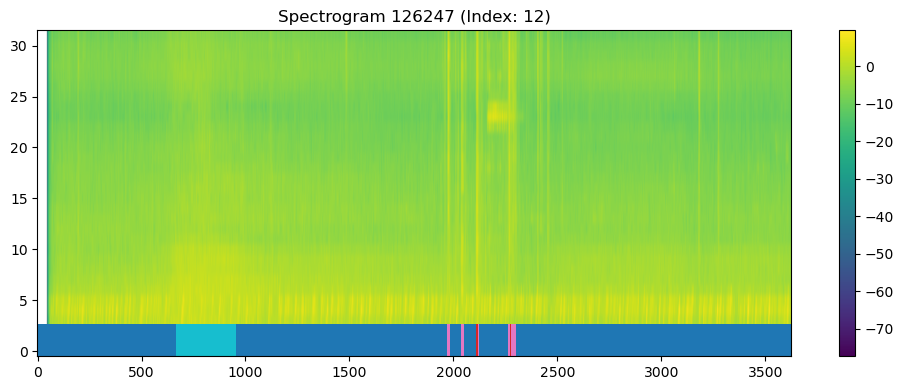
\includegraphics[width=\linewidth]{img/train_spectrogram_12_kmeans.png}
\end{minipage}

\vspace{1em}

\begin{minipage}{0.6\linewidth}
\textit{DBSCAN}: a density-based method capable of automatically determining the number of clusters, however, tweak epsilon and min size.
\end{minipage}
\hfill
\begin{minipage}{0.35\linewidth}
  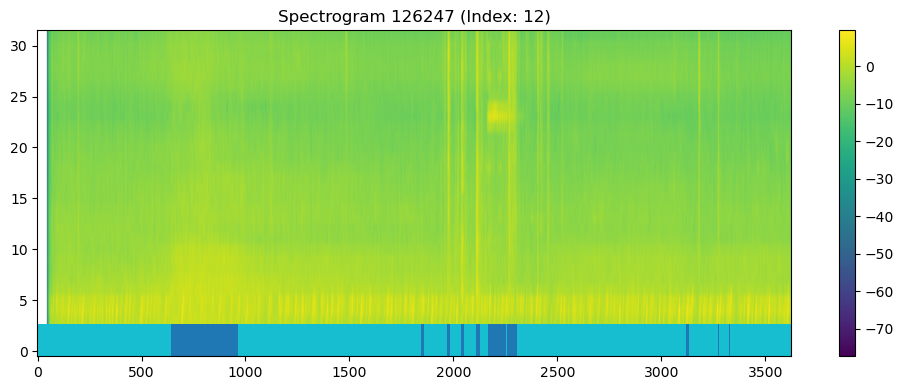
\includegraphics[width=\linewidth]{img/train_spectrogram_12_dbscan.png}
\end{minipage}

At a first glance, we noticed that clustering produced extremely thin and 'dispersed' groupings. In order to enforce wider windows, we also experimented with different ways to enforce continuity of the clusters in time: first encouraging time continuity by adding the time index to the data as an additional column, and second by experimenting with enforcing it as a hardcoded constraint. In both cases, we were unable to produce distinct results that could be usable for an initial filtering. While parameter tuning could yield reasonable clusters in individual cases, the method's performance degraded significantly across recordings with different background conditions or device setups.

In all cases, we were unable to refine the clusters parameters to work over multiple audio files. As a resutl, we concluded that clustering methods are ineffective for isolating bird calls from raw audio, particularly in unlabeled data. Given their limited robustness and generalization, we moved to exploring alternative ways of extracting animal calls, detailing our methods in the following sections.

\subsection*{Rating-Based Filtering}

We first leveraged the rating system available in the Xeno-Canto dataset:

\begin{itemize}
  \item Analyzed the distribution of ratings, finding most clips rated above 3.5
  \item Identified that filtering out low-rated samples (< 3.5) would affect only 0.19\% of the data
  \item Found two species (Jaguar '41970' and Spotted Foam-nest Frog '126247') that would be lost if excluded by rating.
  \item Implemented a preservation strategy by retaining the top 5 highest-rated examples of at-risk species.
\end{itemize}

\subsection*{YAMNet Audio Classification}

Since rating-based filtering only affected a small portion of our dataset, and since we wanted to better navigate the variety of nature of the spliced audio clips, we sought a pre-trained deep learning model for audio classification. We identified Google's YAMNet model,  based on the AudioSet dataset. YAMNet can identify the main category of sound in a clip out of a comprehensive list of 521 event classes, which enabled us to automatically annotate and filter clips based on their primary acoustic content.

We applied YAMNet filtering with the following procedure:

\begin{enumerate}
  \item \textbf{Segmentation}: All recordings were split into the standardized 5 sec clips, aligning with the input format required for our downstream models
  \item \textbf{Classification}: Each segment was passed through YAMNet to obtain a predicted label from the 521 available event classes.
  \item \textbf{Curated "Keep" List}: We created a whitelist, "All", of 27 relevant audio classes, including such categories as "Bird", "Animal", and other ecologically meaningful sounds, to priotize \textit{data quality}. The filter retained 67\% of the training set, losing 6 classes out of 206.
  \item \textbf{Curated "Remove" List}: We also created a list, "Light", to maintain \textit{data quantity}, where a more lenient regime removed only the largest present, and most clearly irrelevant classes: "Silence", "Noise", "Vehicle". This filter retained 83\% of the training set.
  \item \textbf{Validation}: Verified that the filtering preserved broad species representation across the dataset.
\end{enumerate}

\begin{minipage}{0.48\linewidth}
This two-stage approach allowed us to produce different refinements of the dataset with an improved quality in the data, while maintaining the label diversity. The remaining audio segments were cleaner and more relevant for model training. Consequently, we hoped that the step would improve classification performance.
\end{minipage}
\hfill
\begin{minipage}{0.48\linewidth}
  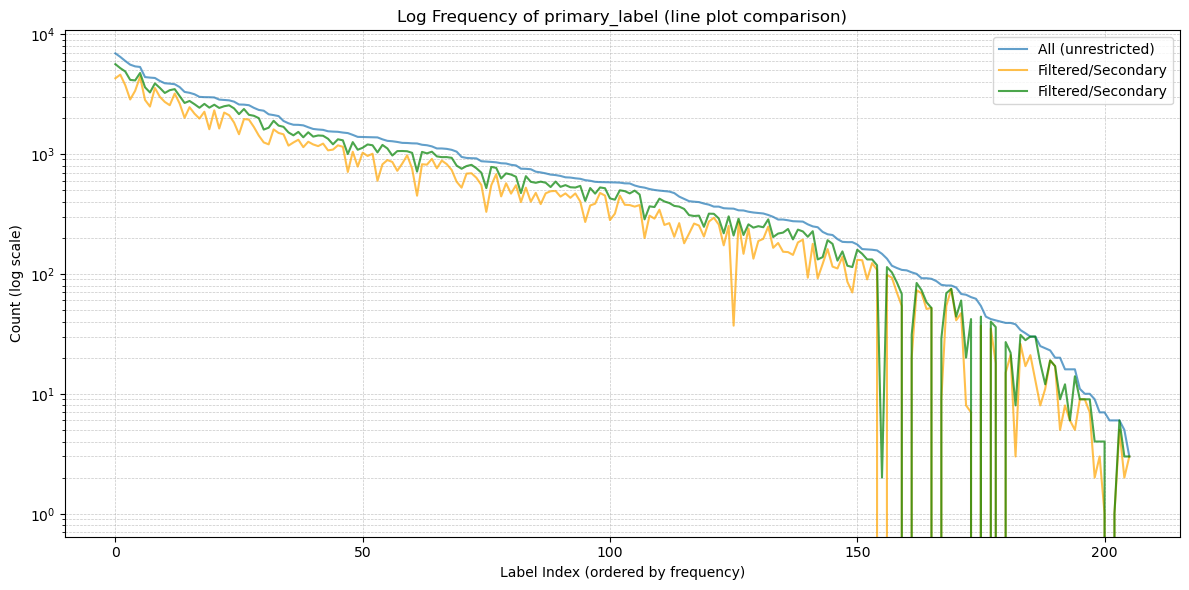
\includegraphics[width=\linewidth]{img/primary_yamnet_filtering.png}
\end{minipage}


\subsection*{Data Augmentation}

To improve generalization and robustness in our models, we applied multiple spectrogram augmentation techniques during training. We leveraged both labeled and unlabeled audio data to increase variability and mitigate class imbalance. The augmentations included:

\begin{enumerate}
  \item \textbf{SpecAugment-based Transformations} \cite{specaugment}
    \begin{itemize}
      \item \textit{Time masking}: Random horizontal stripes (time axis) were zeroed to simulate occluded temporal segments.
      \item \textit{Frequency masking}: Random vertical stripes (frequency axis) were zeroes to simulate missing spectral bands.
      \item \textit{Random brightness and contrast adjustments}: Gain and bias varied to simulate different recording conditions, intensity clamped to a normalized [0, 1] range.
    \end{itemize}

  \item \textbf{Mixup Augmentation} \cite{mixup_survey}

    Input batches were augmented using the Mixup technique, where pairs of samples were linearly interpolated:
    \begin{itemize}
      \item Spectrograms were combined as $\tilde{x} = \lambda x_1 + (1 - \lambda) x_2$ with $\lambda$ sampled from a Beta distribution.
      \item Targets were mixed proportionally to $\lambda$.
      \item The loss function was adjusted accordingly to interpolate between the two labels.
    \end{itemize}

  \item \textbf{Labeled-Unlabeled Interpolation}

    To exploit the large pool of unlabeled data, we generated synthetic training examples by interpolating the mel spectrogram of a labeled recording with that of a uniformly sampled unlabeled clip.
\end{enumerate}

\subsection*{Label Smoothing}

To take advantage of the information provided by the secondary labels, we modified the target label distribution used during training. Specifically, we constructed soft target probability vectors by distributing label mass between the primary label and its associated secondary labels, controlled by a parameter $m \in [0,1]$. We started from one-hot encoding of the primary label, taken as the basis vector $\mathbf{e}_m$, which we scaled by $m$, adding to it the encoding vectors as the uniform probability of the secondary labels: $\frac{1-m}{\#\text{secondary labels}}$ for each possible secondary label. Finally, we included a 'null' label in the classifier, to account for lower confidence levels and allow the network to provide null labels. In data points without secondary labels, the leftover probability mass was placed in the 'null' label, to ensure the probability vector was consistent.

\section*{Modelling and Experiments}

We built towards the task of soft classification using models of increasing complexity, before comparing the results with a state-of-the-art solution, which we extended with data augmentation. It should be noted that the baseline accuracy of a model guessing randomly, given the distribution of the data, is $\text{P}_\text{correct} = 0.012$. At this stage of the investigation, we used an 80-20 train-test data split, tracking validation Cross Entropy Loss and Accuracy metrics at the end of every epoch. We used both Loss and Accuracy because loss provided a continuous signal that reflected model confidence and could guide training, even when predictions were incorrect. Accuracy, in contrast, is less informative and only measures the final performance.

\subsection*{MelCNN}

As an initial experiment, we decided to restrict our search to a simple CNN architecture which used only the Mel Spectrogram and was trained from scratch. We studied its performance, using the following performance metrics: Cross Entropy Loss and Accuracy. Compared to the more complex architectures tested later, MelCNN was trained for fewer epochs and with limited data augmentation. The models below explored different values for the label mixing factor $m$ and input filtering strategies.

Performance across configurations varied, but remained poor, with all accuracies falling below 0.05, which indicated both underfitting and general limitations in model capacity. Moreover, although soft labeling ($m=0.8$) on the "All" subset slightly improved accuracy, we noticed that one-hot encoding ($m=1.0$) was more consistently producing higher accuracy, even when extended to 10 epochs. The same appplied for training on the full dataset.

Finally, "Animal" filtering generally performed better than "All" despite fewer training samples, likely due to cleaner or more consistent labelling.

\begin{minipage}{0.48\linewidth}
Empirically, we eventually opted to stop training after 3 epochs, as we saw little improvements in performance after, which we attributed to limited model capacity. After seeing the poor results of this preliminary architecture, we decided to consider a more complex model, trained for a longer time, in order to improve generalization and achieve higher accuracies.
\end{minipage}
\hfill
\begin{minipage}{0.48\linewidth}
\centering
\begin{tabular}{|l|r|r|r|l|}
\hline
Data  & Epochs & Encoding & Accuracy & Hash     \\
\hline
All    & 10     & 1.0      & 0.0298   & c580a9c1 \\
All    & 3      & 1.0      & 0.0261   & c580a9c1 \\
Light  & 3      & 1.0      & 0.0397   & c580a9c1 \\
All    & 3      & 1.0      & 0.0261   & 5a6176d1 \\
Light  & 3      & 0.8      & 0.0402   & 5a6176d1 \\
\hline
\end{tabular}
\end{minipage}
\subsection*{EfficientNet}

After our limited successes in training models from scratch, we opted to try a different approach: applying \emph{transfer learning} and filtering the datasets as little as possible \cite{efficientnet}.

As an initial step, we tested the model's ability to fit to the data, observing a high training accuracy ($0.77$ and $0.76$) on both All and Light datasets with one-hot encoding ($m=1.0$). As expected, taking more data corresponded to obtaining a higher accuracy, and these models significantly surpassed the baseline.

\begin{table}[h!]
  \centering
  \begin{tabular}{|l|r|r|r|l|}
    \hline
    Data  & Epochs & Encoding & Train Acc. & Hash     \\
    \hline
    All    & 15     & 1.0      & 0.770     & c580a9c1 \\
    Light  & 15     & 1.0      & 0.760     & 9964eb55 \\
    \hline
  \end{tabular}
  \label{tab:train_results}
\end{table}

Small gap between All and Light datasets suggested that both contain enough learnable patterns, and EfficientNet is robust across them. We then considered a much larger parameter class, varying the number of epochs, the encoding value $m$ and observing accuracy metrics.

\begin{table}[h!]
  \centering
  \begin{tabular}{|l|c|r|r|c|l|}
    \hline
    Data  & Epochs & Encoding & Accuracy & Bal Acc & Hash     \\
    \hline
    All   & 10     & 1.0      & 0.476    & /       & 8b600946 \\
    All   & 10     & 0.8      & 0.451    & /       & 8b600946 \\
    Light & 8/10   & 1.0      & 0.315    & /       & 781592e6 \\
    Light & 6/10   & 0.8      & 0.266    & /       & 781592e6 \\
    All   & 10     & 1.0      & 0.498    & 0.400   & 0a242441 \\
    All   & 6/10   & 0.7      & 0.343    & 0.304   & 0a242441 \\
    \hline
  \end{tabular}
  \label{tab:balanced_accuracy}
\end{table}

Through the experiments, we noticed clear signs of overfitting: the model reached a training accuracy of about 0.77, but its evaluation accuracy on the same dataset (with hard labels, m=1.0) was significantly lower at 0.476. This gap suggests the model may learn patterns that don't generalize well, even on familiar data. We also tested soft labeling by adjusting the label confidence to $m=0.8$, which slightly decreased performance, by producing an evaluation accuracy of 0.451. Once more, we observed that in the setup, soft labeling hurts performance, potentially, as it introduces uncertainty or emphasizes less confident predictions, which confuses the model. To reduce noise in the dataset, we applied a filtering step using Light Yamnet, which resulted in a noticeable drop in accuracy compared to using the full dataset. Filtering may have reduced noise, albeit at the cost of losing signal diversity, necessary for the model to generalize better. When we combined filtering with soft labeling, performance degraded even further. This aligns with the idea that soft supervision might not be effective when the dataset is already sparse or contains weak signals. Adding uncertainty in such cases can be more harmful than helpful. Overall, the best performance (val\_acc = 0.498) was achieved when using the full dataset with hard labels (m=1.0). This supported the conclusion that, for our setup, full supervision with confident labels is the most effective approach. Finally, we found that very soft labels (m=0.7) combined with early stopping (after 6 out of 10 training epochs) led to a significant drop in both accuracy (down to 0.343) and balanced accuracy (0.304). This further highlights how sensitive the model is to supervision quality and training strategy.

\subsection*{Takeaways}

\begin{minipage}{0.48\linewidth}

In our training experiments, we considered $\text{m} \in \{0.7, 0.8, 1.0\}$, yet we always observed better results with $\text{m} = 1$, that is, one-hot encoding. A simple model like the MelCNN was not able to capture the full image of the data, which was particularly clear when observing the much higher accuracy score of the EfficientNet variation. Given the limited amounts of data, overfitting was a real concern, warranting the use of more sophisticated techniques to avoid it, notably Balanced Accuracy and Cross-Fold validation.
\end{minipage}
\hfill
\begin{minipage}{0.48\linewidth}
  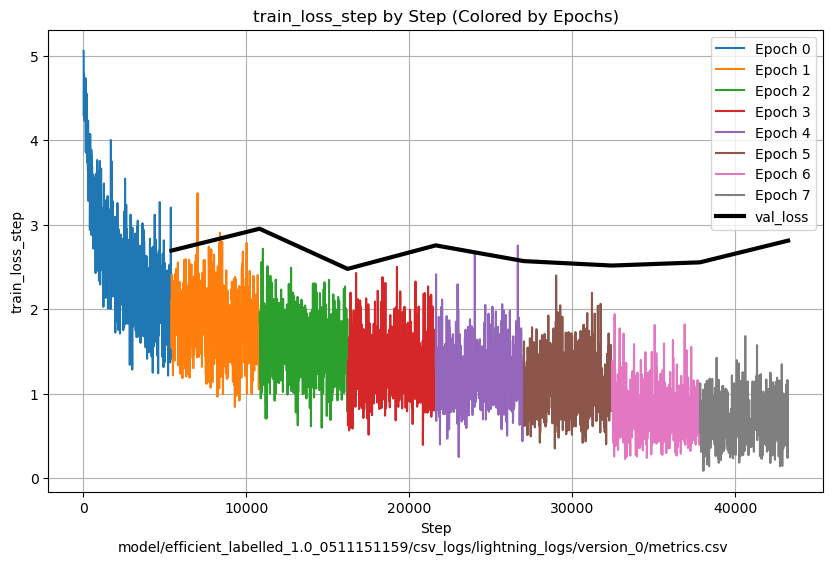
\includegraphics[width=\linewidth]{img/efficient_loss_accuracy_plot.png}
\end{minipage}


\section*{Comparison to SOTA EfficientNet Implementation}

In line with our observations on the exploratory models, we addressed shortcomings and limitations by comparing the results of our implementation with those of a State-Of-The-Art solution. To address class imbalances, since some classes appear far more frequently than others, we resorted to Balanced Accuracy. This metric computes the average of recall (true positive rate) for each class, ensuring that all classes contribute equally to the final score, regardless of their frequency in the dataset. We use the following key metrics are used to evaluate model performance: Binary Cross Entropy Loss, Balanced Accuracy, and AUC Score. Binary Cross Entropy Loss is a standard loss function for binary classification tasks that measures the distance between predicted probabilities and actual binary labels. It penalizes incorrect predictions with high confidence more heavily, encouraging the model to output calibrated probabilities. AUC Score, or Area Under the Receiver Operating Characteristic Curve, evaluates the model's ability to distinguish between classes across all possible thresholds, offering a threshold-independent view of performance. Finally, we used cross-validation to reduce the risk of overfitting on the data during the training phase. This was also relevant in training the final, complete model on the whole dataset, as a 100-0 split would have lacked a reliable accuracy metric to decide when to stop the training.

\subsection*{Results}

\begin{minipage}{0.60\linewidth}
Observing the evolution of loss throughout training, we noticed a similar phenomenon to the previous implementation of EfficientNet: the model is slow to generalize, despite the advantages of the new configuration, and the availability of the full training dataset.
\end{minipage}
\hfill
\begin{minipage}{0.35\linewidth}
  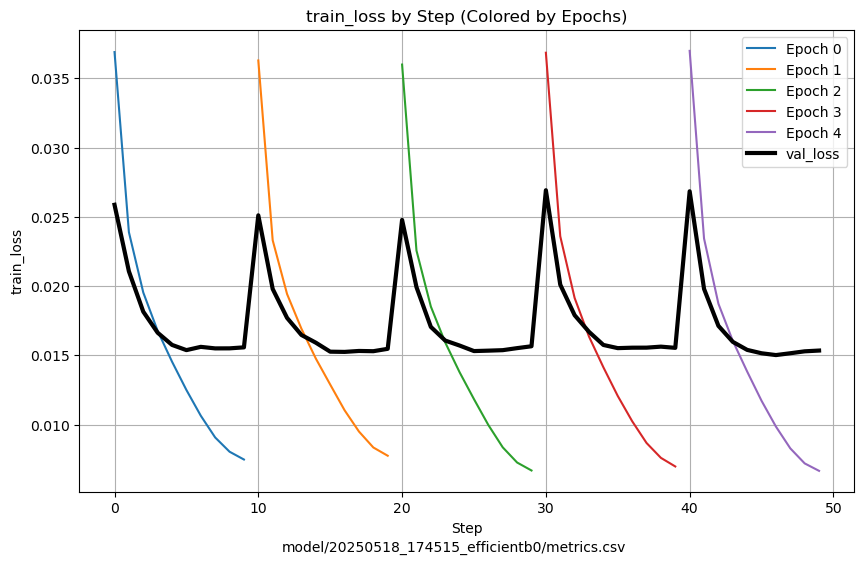
\includegraphics[width=\linewidth]{img/efficientb_loss_kfold.png}
\end{minipage}

\vspace{1em}

\begin{minipage}{0.6\linewidth}
On a second note, validation accuracy fell within the previous results, though it was higher as a result of the enlarged training data. This could be attributed to K-fold cross-validation training on the whole dataset, as opposed to only 80\% of it.
\end{minipage}
\hfill
\begin{minipage}{0.35\linewidth}
  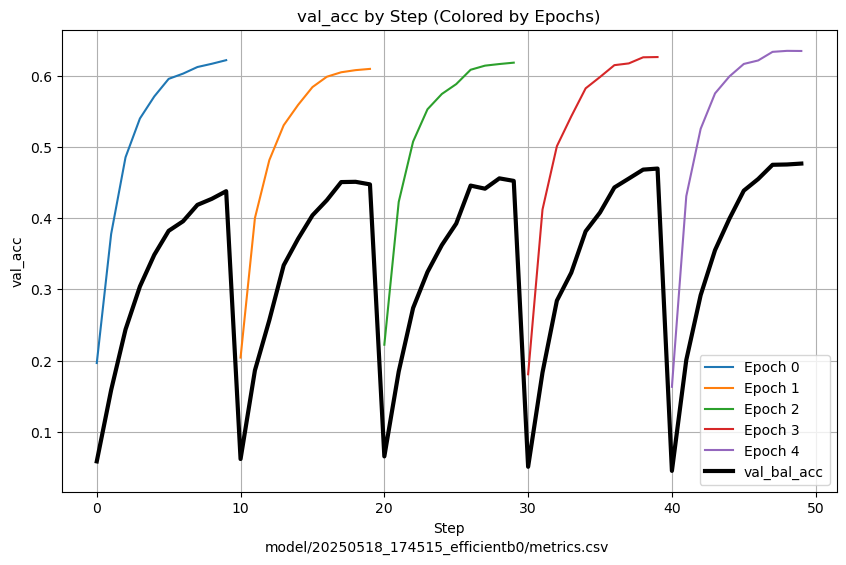
\includegraphics[width=\linewidth]{img/efficientb_acc_kfold.png}
\end{minipage}

\begin{minipage}{0.6\linewidth}
To account for the limitations of cross-validation, we also trained a model using the same regime for 90\% of the dataset, validating at the end on 10\% of the dataset. Plotting the confusion matrix, there is no clear 'bias' between taxonomy groups: the model performs uniformly over different labels. For reference, the new model performed with 0.78 accuracy when using the whole train dataset (hash 59672068). 
\end{minipage}
\hfill
\begin{minipage}{0.35\linewidth}
  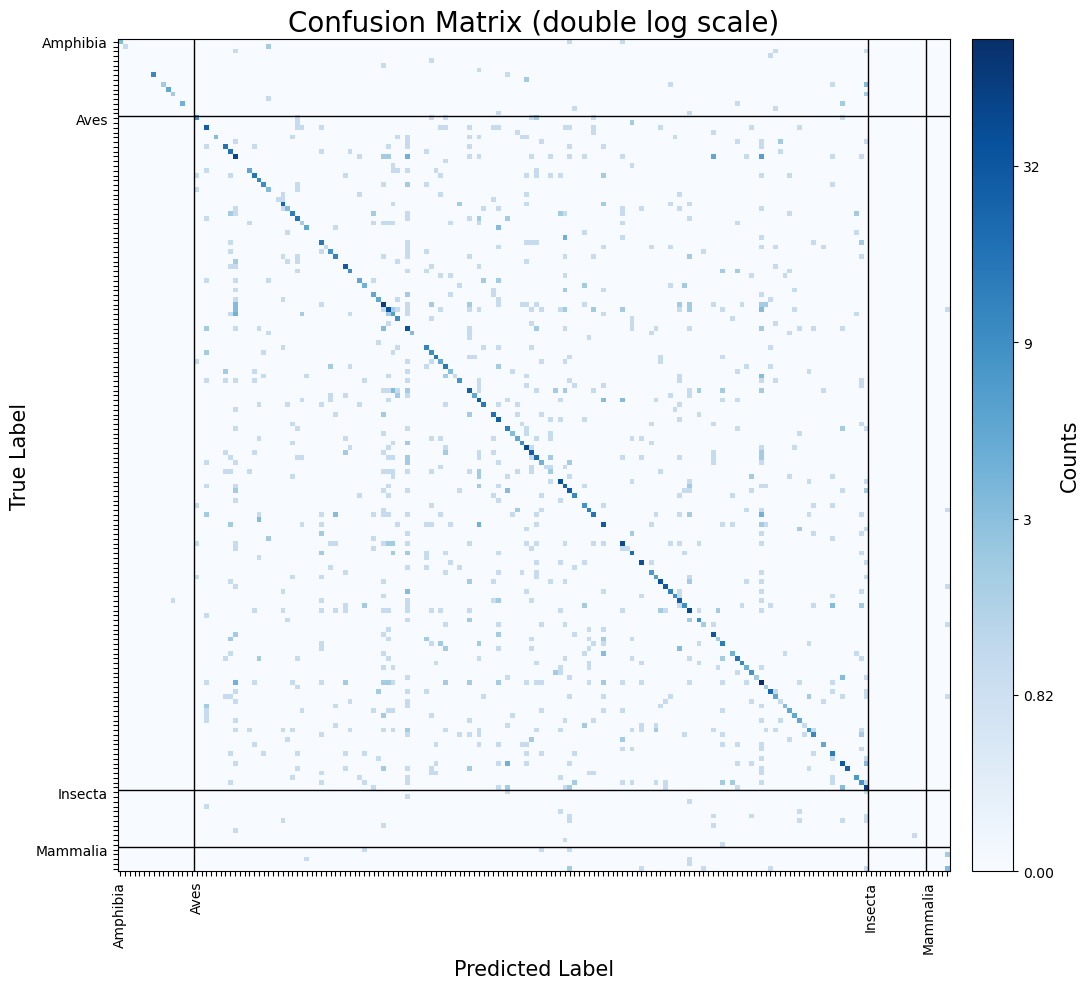
\includegraphics[width=\linewidth]{img/confusion_matrix_efficientb_train.png}
\end{minipage}

\section*{Semi-supervised Learning}
Given the vast amounts of unlabeled audio recordings that were also present in the dataset, we attempted to use semi-supervised learning to improve the model: we first added labels to the soundscape recordings using our best performing model, before continuing to train the model on the newly generated labels. We hoped that the additional training might provide the model with more information on the distribution of the dataset, potentially improving its performance.

\begin{minipage}{0.65\linewidth}
As an additional note, we also ran the "naive" EfficientNet implementation, comparing the labelling of the two with the help of a confusion matrix. We observed prominent vertical and horizontal streaks in the plot, which is consistent with the expectations: as the old model was biased and somewhat overfitted, we could identify in vertical lines labels that were clumped by the naive implementation but differentiated in the new model, and the opposite in the horizontal lines: uncertain labellings which belonged to a single class according to the newer model.
\end{minipage}
\hfill
\begin{minipage}{0.30\linewidth}
  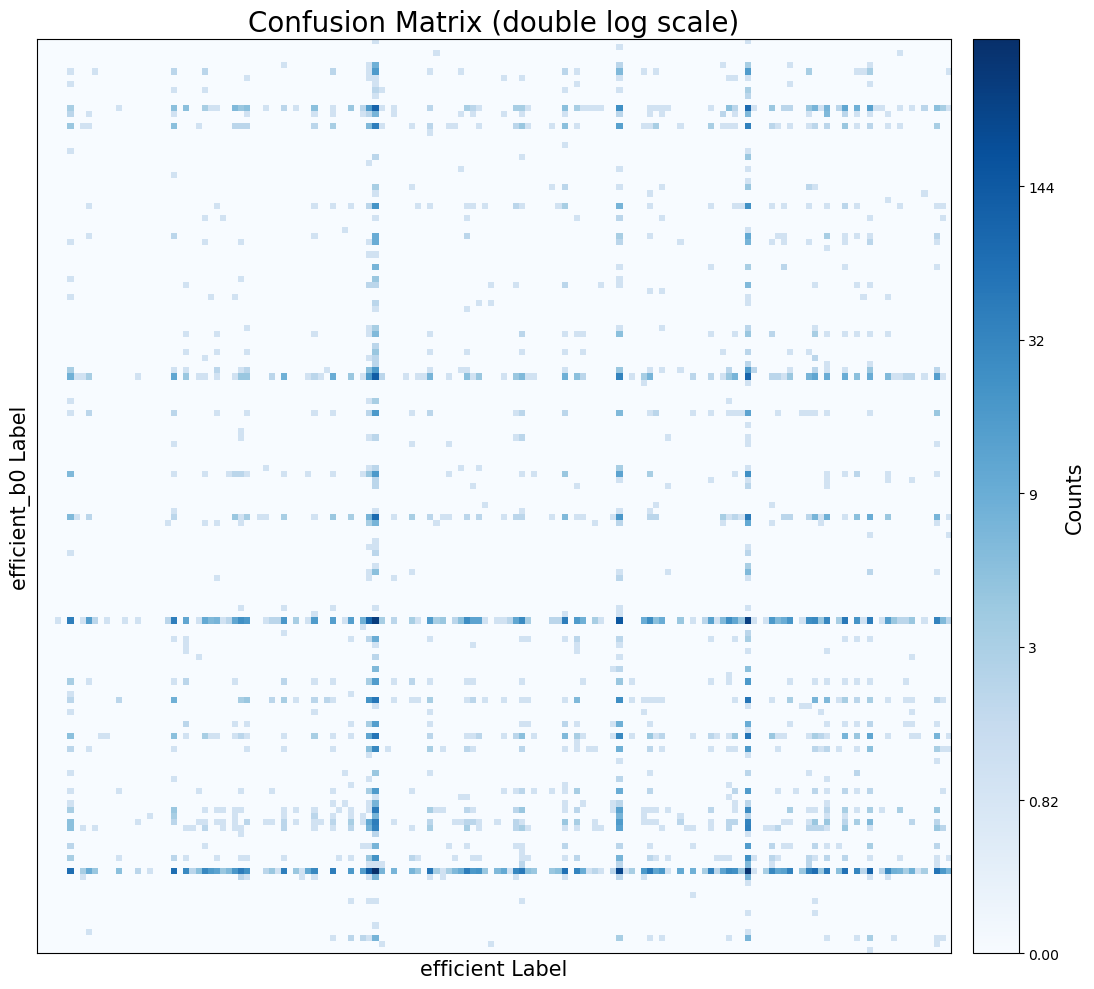
\includegraphics[width=\linewidth]{img/confusion_matrix_efficient_models.png}
\end{minipage}

\vspace{1em}

\begin{minipage}{0.65\linewidth}
Plotting the training performance for the second stage of training, we observed more 'spikey' accuracy, which could be attributed to overfitting. Moreover, through variations of the model, we noticed that the performance generally peaked in the second fold, taking different models.
\end{minipage}
\hfill
\begin{minipage}{0.30\linewidth}
  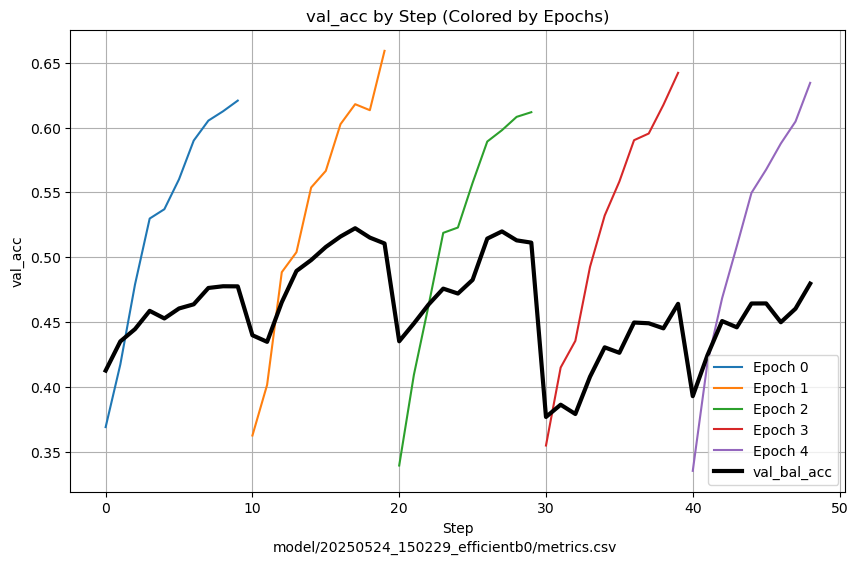
\includegraphics[width=\linewidth]{img/semisuper_learning_val_acc.png}
\end{minipage}

\subsection*{Kaggle Scoreboard}

To compare the final performance of the models, we used Kaggle's hidden test feature, since the full model was trained on the complete dataset, leaving no data for the validation step.

\begin{minipage}{0.48\linewidth}
We tracked the effect of various training changes to accuracy: augmenting underrepresented classes, running Curriculum Learning \cite{curriculum_learning} with the Soundscapes and taking different stages throughout the training phase of the model. In general, we saw worse performance when augmenting underrepresented classes. This effect was particularly obvious when training on the original train dataset. Moreover, later folds of training on the soundscape dataset performed worse (commit hash 6f4a47ac).
\end{minipage}
\hfill
\begin{minipage}{0.48\linewidth}
\centering
\begin{tabular}{|l|c|l|r|}
\hline
\textbf{Soundscape} & \textbf{Fold} & \textbf{Augmentation} & \textbf{AUC} \\
\hline
No         & 5    & No               & 0.781 \\
No         & 5    & Yes              & 0.500 \\
Yes        & 1    & Yes (soundscape) & 0.728 \\
Yes        & 1    & No               & 0.725 \\
Yes        & 5    & No               & 0.717 \\
\hline
\end{tabular}
\end{minipage}

We were unsuccessful at improving the performance of the model beyond the state-of-the-art model: no variation on the new model improved the performance. We attribute this to the dataset, which has shown itself to be sensitive to changes both in training and data.

\section*{Evaluation of Methodology}

The code for the investigation was developed in Python, using a mix of Python scripts and Jupyter notebooks depending on our need for interactivity. For instance, model scripts were written as \texttt{.py} files, while exploratory graphs and one-time data operations were handled in interactive notebooks. Once specifc notebook code blocks reached maturity, we exported them to standalone scripts. Version control was managed using Git, with the repository hosted on GitHub. Overall, we were satisfied with this structure.

We performed less intensive operations on our personal laptops, such as coding or test-running the models on a small batch of the data. On the other time, training and other data-heavy tasks were automated using shell scripts, which were submitted to the High Performance Cluster (HPC) available to us through our university, \textit{Università Commerciale Luigi Bocconi}\cite{unibocconi}. We relied on shell utilities for most data transfers between our local devices and the HPC, referencing results by their Git commit hash for reproducibility.

Initially, we experimented with different models and introduced flexible hyperparameter configurations to increase generality. Eventually we found ourselves developing two models (MelCNN and EfficientNet), while only being seriously interested in one of them, which consumed time that would have been better spent developing new models. In hindsight, a more solution-oriented, version history, ie. keeping the code lighter and hardcoding more variables, would have been more time efficient.

We tracked our efforts using custom time-tracking tools: the org-mode library \cite{doom_emacs} in Emacs \cite{gnu_emacs} and Clockwork \cite{clockwork}, an independently developed productivity utility. The bulk of the project was completed in approximately 100 hours over the course of six weeks, which produced over 150 commits.

\section*{Conclusion}
This study investigated machine learning approaches for species classification in the BirdCLEF2025 challenge, evaluating the challenges of extreme class imbalance and limited labeled data. While clustering proved ineffective for segmentation, we evaluated MelCNN and EfficientNetB0 architectures, ifnding the latter significantly more effective. Attempts to refine the dataset and incorporate soft labels did not yield consistent improvements. As a successive step, we implemented semi-supervised learning, adding pseudo-labels to the unlabeled soundscape data and continuing training of a model for a different number of times and data augmentation for underrepresented labels. Despite these efforts, we failed to improve performance beyond the baseline, with our best model achieving 0.781 accuracy on the Kaggle scoreboard. While we did not surpass state-of-the-art performance, this comprehensive analysis provides insights into the challenges of ecological audio classification and demonstrates that traditional techniques may not transfer effectively to highly imbalanced ecological datasets, suggesting future research should focus on few-shot learning and domain-specific methods tailored to biodiversity monitoring applications.

\newpage

\begin{thebibliography}{10}

\bibitem{birdclef2025}
BirdCLEF 2025 -- Kaggle Competition. \url{https://www.kaggle.com/competitions/birdclef-2025} (accessed June 1, 2025).

\bibitem{mel_cepstrum}
Mel-frequency cepstrum. \url{https://en.wikipedia.org/wiki/Mel-frequency_cepstrum} (accessed June 1, 2025).

\bibitem{efficientnet}
EfficientNet -- Wikipedia. \url{https://en.wikipedia.org/wiki/EfficientNet} (accessed June 1, 2025).

\bibitem{specaugment}
SpecAugment: A Simple Data Augmentation Method for Automatic Speech Recognition. \url{https://arxiv.org/abs/1904.08779} (2019).

\bibitem{mixup_survey}
Mixup Augmentation - A survey on Image Data Augmentation for Deep Learning. \url{https://journalofbigdata.springeropen.com/articles/10.1186/s40537-019-0197-0} (2019).

\bibitem{curriculum_learning}
Curriculum Learning -- Wikipedia. \url{https://en.wikipedia.org/wiki/Curriculum_learning} (accessed June 1, 2025).

\bibitem{unibocconi}
Università Commerciale Luigi Bocconi. \url{https://www.unibocconi.it/it} (accessed June 1, 2025).

\bibitem{clockwork}
ClockWork by Tommaso Ferracina -- GitHub. \url{https://github.com/quercia-dev/Attimo} (accessed June 1, 2025).

\bibitem{gnu_emacs}
GNU Emacs -- Official Site. \url{https://www.gnu.org/software/emacs/} (accessed June 1, 2025).

\bibitem{doom_emacs}
Doom Emacs Configuration by Tebe Nigrelli -- GitHub. \url{https://github.com/tebe-nigrelli/doomemacs-config} (accessed June 1, 2025).

\end{thebibliography}

\end{document}